\documentclass[report.tex]{subfiles}
\begin{document}

This chapter presents the data of the experiments described above.
Information about the system that ran them, as well as the full data from
the experiments themselves as are available in Appendix
\ref{app:experiment}.

All experiments have been executed 10 times, and the results reported here
are accumulations of the prediction accuracies and errors.
Because all layers uses a constant seed in Futhark, the results are constant and
standard deviations have been omitted.
The experiments use a 80/20 training/testing split. 

\section{NAND}

Data from the NAND experiment is shown in Table \ref{tab:xor}.
The rates are below chance levels in NEST, both during
the random weight initialisation and while transferring weights from Futhark.

\def\arraystretch{1.2}%  1 is the default, change whatever you need
\begin{table}
  \begin{tabular}{r|l l}
  \label{tab:nand}
  Backend & Random weights & Transferred weights \\ \hline
  Futhark & 1 & - \\
  NEST & 0.37 $\pm$ 0.040 & 0.69 $\pm$ 0.216\\ 
  BrainScaleS & - & -
  \end{tabular}
  \caption{Mean accuracies and standard deviations the NAND experiment.}
  \label{tab:xor}
\end{table}

\begin{figure}
  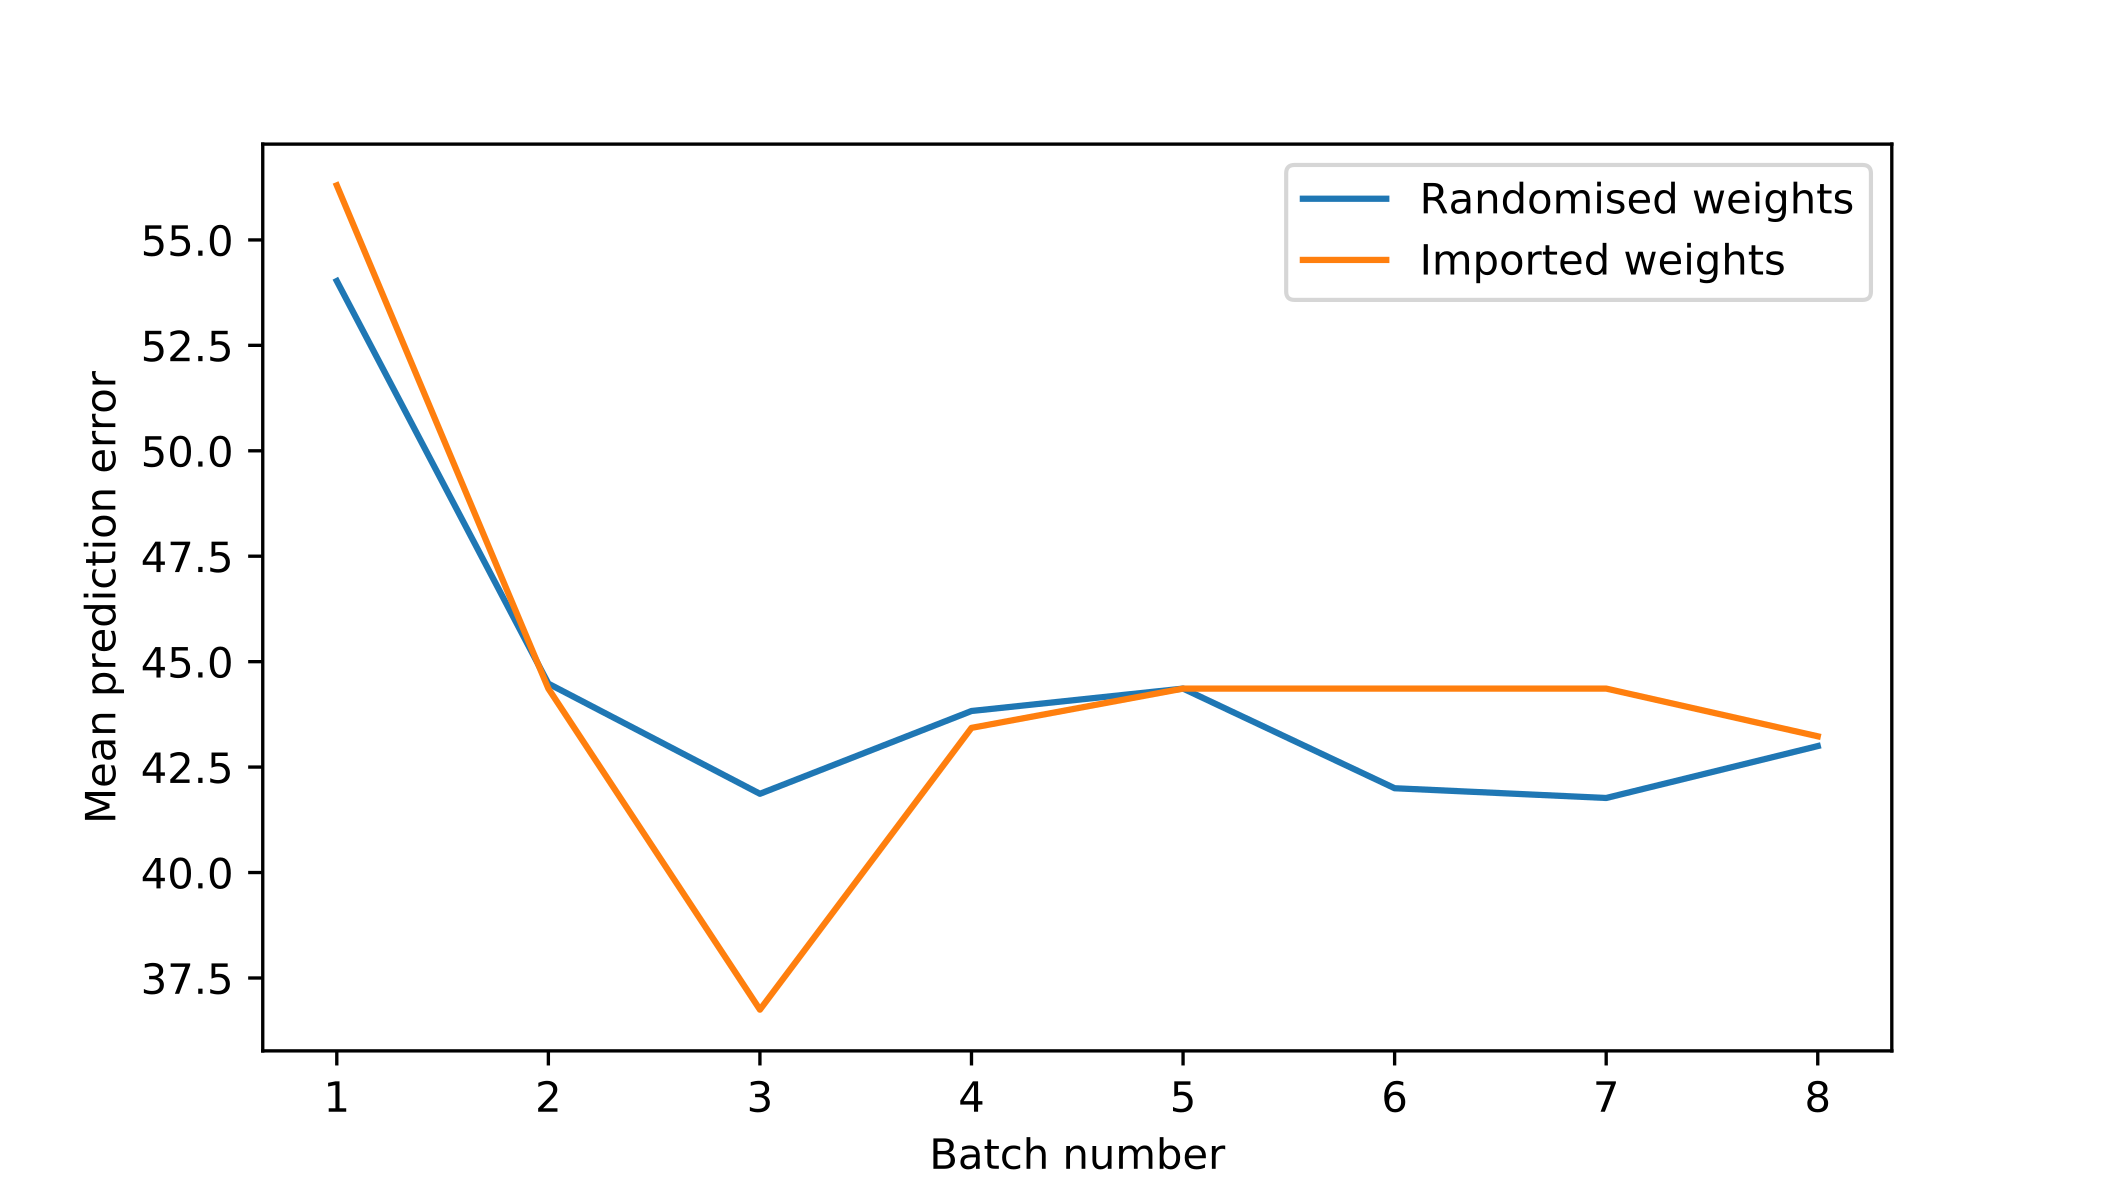
\includegraphics[width=\linewidth]{images/nand.png}
  \caption{Summed error rates for the NAND network simulated in NEST. The rates
  are produced following each batch and are averaged over 10 simulations.}
  \label{fig:nand_snn}
\end{figure}
\FloatBarrier

\section{XOR}

Tabel \ref{tab:nand} shows the NAND experiment results. 
\begin{table}
  \begin{tabular}{r l l}
  Backend & Random weights & Transferred weights \\ \hline
  Futhark & 1.000 & - \\ 
  NEST & 0.530 $\pm$ 0.038 & 0.585 $\pm$ 0.033 \\
  BrainScaleS & -
  \end{tabular}
  \caption{Mean accuracies and standard deviations for the XOR experiment.}
  \label{tab:nand}
\end{table}

\begin{figure}
  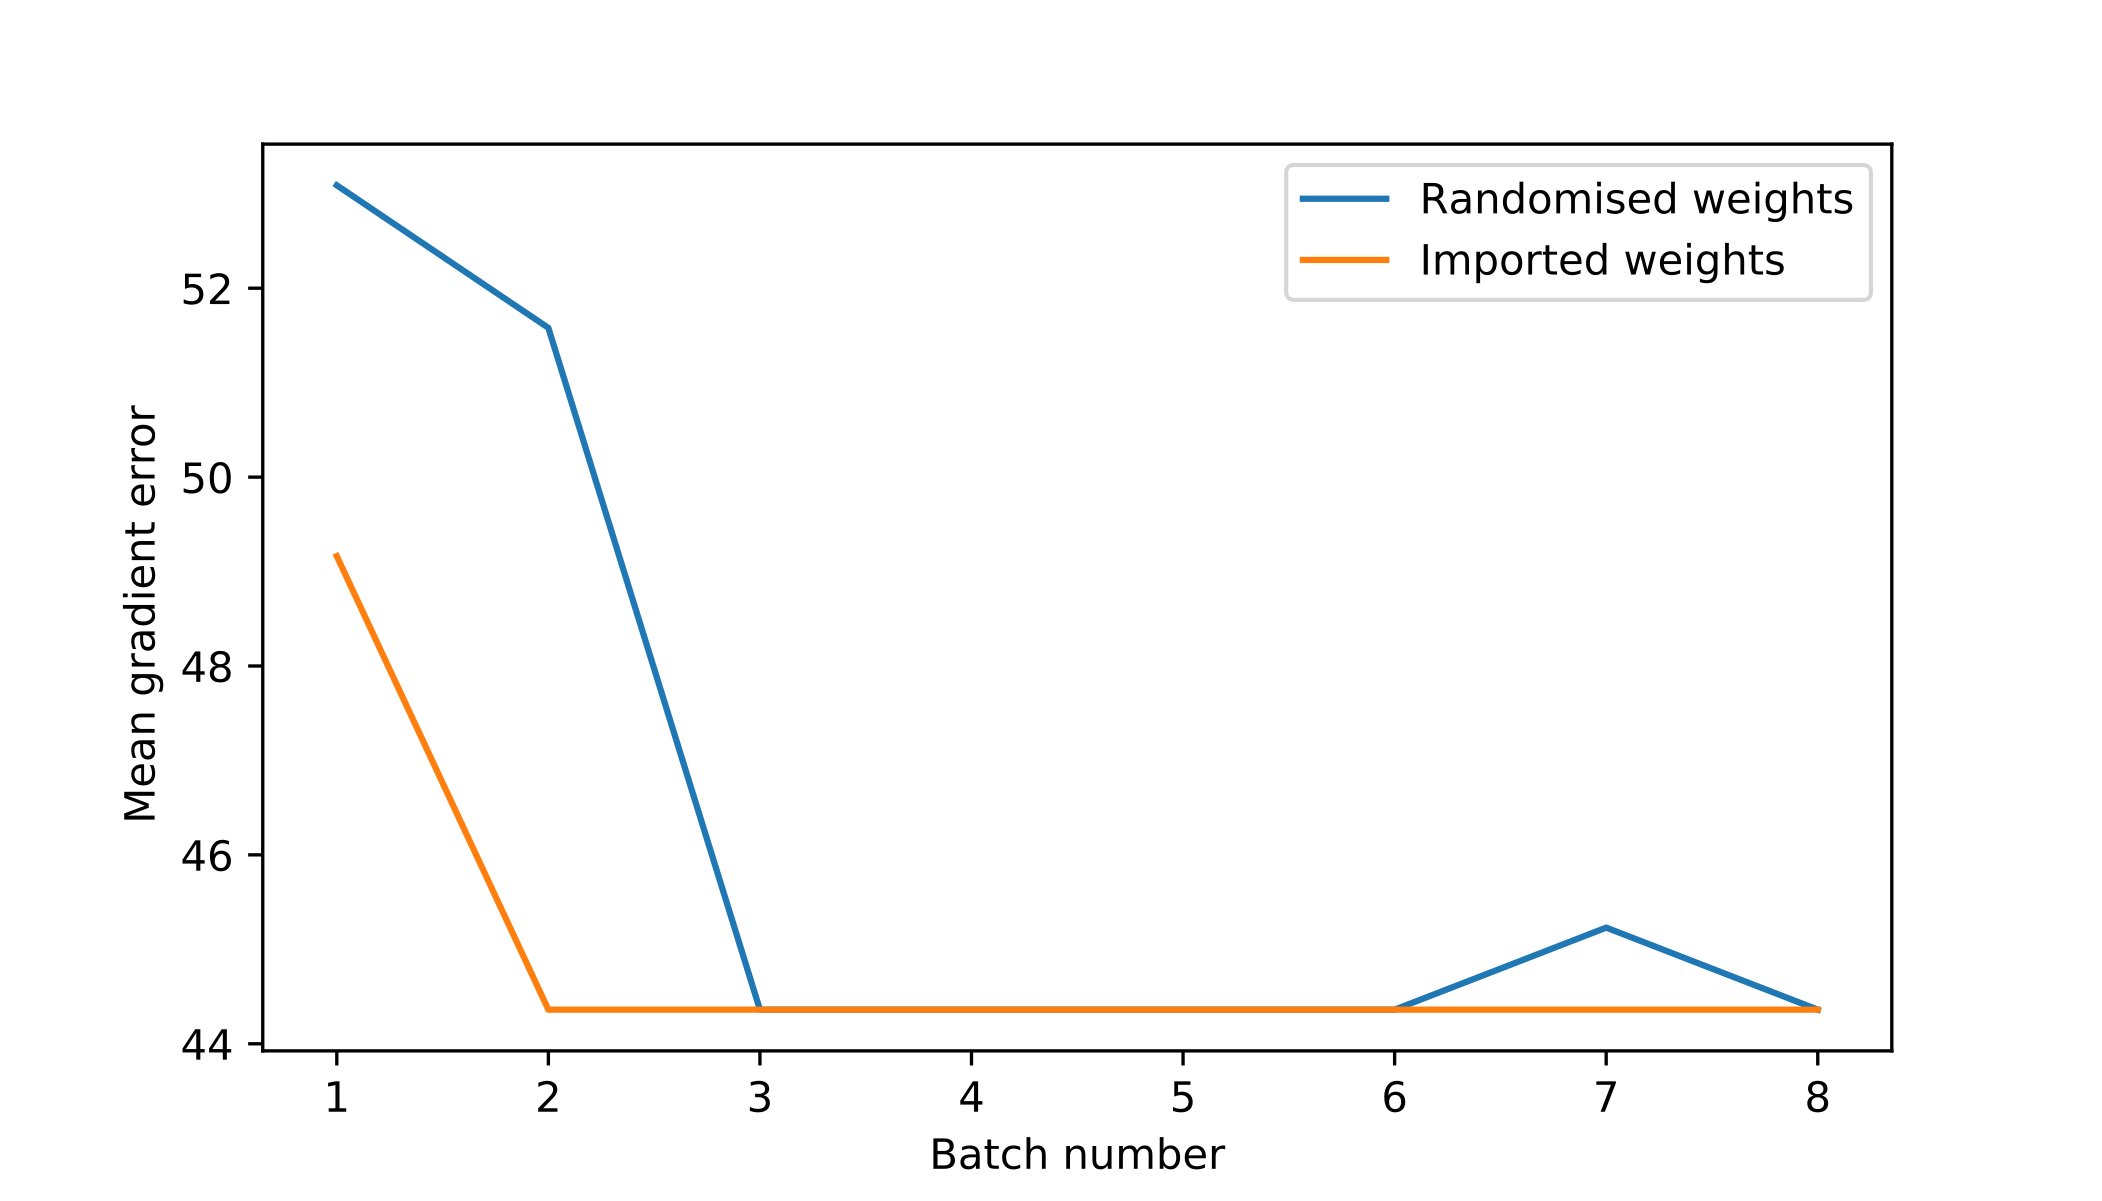
\includegraphics[width=\linewidth]{images/xor.png}
  \caption{Summed error rates for the XOR network simulated in NEST. The rates
  are produced following each batch and are averaged over 10 simulations.}
  \label{fig:xor_snn}
\end{figure}

\FloatBarrier

\section{MNIST}

\begin{table}
  \begin{tabular}{r l l}
  Backend & Random weights & Transferred weights \\ \hline
  Futhark & 0.710 & - \\ 
  NEST & $\pm$ & $\pm$ \\
  BrainScaleS & -
  \end{tabular}
  \caption{Mean accuracies and standard deviations for the MNIST sequential experiment.}
  \label{tab:nand}
\end{table}
\end{document}
